\documentclass[../../main.tex]{subfiles}
\begin{document}

{\bf [解]}
\paragraph{(1)}

% TODO: 概要図
% TODO: 概要図 (修正版: 三角形実線化・重なり解消・theta追加・d単体削除)
\begin{figure}[htb]
  \centering
  \begin{tikzpicture}[scale=1.9, >=stealth, every node/.style={font=\small}]

    % ============================================================
    % 1. 座標定義 (1辺 L = 3.0 の正三角形)
    % ============================================================
    \coordinate (O)  at (0, 0);
    \coordinate (A1) at (0, 1.732);
    \coordinate (A2) at (-1.5, -0.866);
    \coordinate (A3) at (1.5, -0.866);

    % ============================================================
    % 2. 正三角形の外枠 (実線に変更)
    % ============================================================
    \draw[line width=1.1pt, gray!50!black] (A1) -- (A2) -- (A3) -- cycle;
    \node[below=3pt, font=\scriptsize, gray!60!black] at (0, -0.866) {$1\text{辺} = 1000$};

    % 重心・外心 O
    \fill[black] (O) circle (1.3pt) node[right=3pt, font=\footnotesize] {$O$};

    % ============================================================
    % 3. ベクトル a1 = A2 -> A1
    % ============================================================
    \draw[line width=1.5pt, gray!20!black, ->] (A2) -- (A1)
    node[midway, left=4pt, font=\footnotesize\bfseries] {$\vec{a}_1 = \overrightarrow{A_2A_1}$};

    % ============================================================
    % 4. 方向ベクトル e1, e2 および 動点 P1(t), P2(t)
    % 重なりを避けるため、三角形の内側に向かい合って進む自然な幾何配置に設定
    % ============================================================
    % e1: A1 からやや左下へ (角度 -115°)
    % e2: A2 からやや右上へ (角度 30°)
    \coordinate (e1Dir) at ({cos(-112)}, {sin(-112)});
    \coordinate (e2Dir) at ({cos(28)},  {sin(28)});

    % 動点 P1(t), P2(t) の位置
    \coordinate (P1) at ($ (A1) + 1.05*(e1Dir) $);
    \coordinate (P2) at ($ (A2) + 1.25*(e2Dir) $);

    % 軌跡・方向ベクトル e1, e2 の描画
    \draw[dashed, red!60, line width=0.8pt] (A1) -- (P1);
    \draw[line width=1.4pt, red!85!black, ->] (A1) -- ($ (A1) + 0.6*(e1Dir) $)
    node[left=2pt, font=\footnotesize\bfseries, fill=white, inner sep=1pt] {$\vec{e}_1$};

    \draw[dashed, teal!60, line width=0.8pt] (A2) -- (P2);
    \draw[line width=1.4pt, teal!85!black, ->] (A2) -- ($ (A2) + 0.7*(e2Dir) $)
    node[below right=1pt, font=\footnotesize\bfseries, fill=white, inner sep=1pt] {$\vec{e}_2$};

    % ============================================================
    % 5. 動点 P1(t), P2(t) と 最接近距離の線分
    % ============================================================
    \fill[red!85!black] (P1) circle (1.5pt) node[above right=1pt, font=\footnotesize\bfseries] {$P_1(t)$};
    \fill[teal!85!black] (P2) circle (1.5pt) node[below left=1pt, font=\footnotesize\bfseries] {$P_2(t)$};

    % 距離線分 P1-P2 (両矢印)
    \draw[line width=1.4pt, blue!85!black, <->] (P1) -- (P2)
    node[midway, right=3pt, font=\scriptsize\bfseries, fill=white, inner sep=1.5pt]
    {$|\overrightarrow{P_1(t)P_2(t)}| \le 1$};

    % ============================================================
    % 6. 角 theta (相対速度 d = e1 - e2 と a1 のなす角)
    % A2 を始点として相対運動ベクトル d を描画し、a1 との角 theta を明示
    % ============================================================
    \coordinate (dVec) at ($ 0.9*(e1Dir) - 0.9*(e2Dir) $);
    \coordinate (A2_d) at ($ (A2) + (dVec) $);

    % 相対速度方向の補助線 (A2 始点)
    \draw[line width=1.2pt, purple!85!black, ->] (A2) -- (A2_d)
    node[below=2pt, font=\footnotesize\bfseries] {$\vec{d}$};

    % A2 から -d 方向に伸ばす点線（長さを 1.2 倍伸ばす例）
    \draw[dotted, purple!80!black, line width=1.0pt]
    (A2) -- ($ (A2) - 0.6*(dVec) $);

    % a1 の方向角は 60°、dVec の方向角とのなす角 theta を円弧で表示
    \pgfmathsetmacro{\angA}{60}
    \pgfmathsetmacro{\angD}{atan2({sin(-112)-sin(28)}, {cos(-112)-cos(28)})} % d の方向角
    \draw[->, thick, purple!90!black] ($ (A2) + ({0.45*cos(\angA)}, {0.45*sin(\angA)}) $)
    arc (\angA:{\angD + 180}:0.45);
    \node[purple!95!black, font=\footnotesize\bfseries] at ($ (A2) + (0.35, 0.5) $) {$\theta$};

    % ============================================================
    % 7. 頂点ラベル
    % ============================================================
    \fill[black] (A1) circle (1.4pt) node[above=2pt, font=\footnotesize\bfseries] {$A_1$};
    \fill[black] (A2) circle (1.4pt) node[below left=2pt, font=\footnotesize\bfseries] {$A_2$};
    \fill[black] (A3) circle (1.4pt) node[below right=2pt, font=\footnotesize\bfseries] {$A_3$};

  \end{tikzpicture}
  \caption{正三角形 $\triangle A_1A_2A_3$ 上の動点 $P_1(t), P_2(t)$ の運動と最接近条件}
  \label{fig:motion_overview}
\end{figure}

原点$O$からのベクトルを考えると
\begin{align}
  \overrightarrow{OP_k(t)} = \overrightarrow{OA_k} + t \overrightarrow{e_k} \quad (k=1,2,3)
\end{align}
である．また，
\begin{align}
  \vec{d} = \vec{e}_1 - \vec{e}_2 \label{eq:1}
\end{align}
とおく．
$|\overrightarrow{P_1(t) P_2(t)}|$を計算すると
\begin{align}
  |\overrightarrow{P_1(t) P_2(t)}|^2
  &= |\overrightarrow{OP_1(t)} - \overrightarrow{OP_2(t)}|^2 \\
  &= \left| \overrightarrow{A_2 A_1} + t (\overrightarrow{e_1} - \overrightarrow{e_2}) \right|^2 \\
  &= |-\overrightarrow{a_1} + t \vec{d}|^2 \quad (\because{\text{\cref{eq:1}}}) \\
  &= |\overrightarrow{a_1}|^2 + t^2 |\vec{d}|^2 - 2t \vec{a}_1 \cdot \vec{d} \\
  &= 1000^2 + t^2 |\vec{d}|^2 - 2t \cdot 1000 \cdot |\vec{d}| \cdot \cos \theta \quad (0 \le \theta \le \pi)
\end{align}
である．

題意から，これが $1$ 以下になるような $t \ge 0$ があるので
\begin{align}
  & |\vec{d}|^2 t^2 - 2000 \cdot |\vec{d}| \cos \theta \cdot t + 10^6 \le 1 \\
  \therefore
  & |\vec{d}|^2 t^2 - 2000 \cdot |\vec{d}| \cos \theta \cdot t + 10^6 - 1 \le 0
\end{align}
をみたす $t (>0)$ があった．
左辺を $f(t)$ として $f(t)=0$ の判別式 $D$ とすると$|\vec{d}| \ne 0$ からこのような条件は
\begin{align}
  &
  \begin{cases}
    D/4 \ge 0 \\
    0 \le 1000 |\vec{d}| \cos \theta
  \end{cases} \\
  \iff
  &
  \begin{cases}
    10^6 \cdot |\vec{d}|^2 \cos^2 \theta - |\vec{d}|^2 (10^6-1) \ge 0 \\
    0 \le \cos \theta
  \end{cases} \\
  \iff
  &
  \begin{cases}
    (1-\cos^2 \theta) \le \dfrac{1}{10^6} \\
    0 \le \cos \theta
  \end{cases} \\
  \iff
  &
  \begin{cases}
    |\sin \theta| \le \dfrac{1}{10^3} \\
    0 \le \cos \theta
  \end{cases} \label{eq:2}
\end{align}
である．従って $|\sin \theta| \le \dfrac{1}{10^3}$ である．

\paragraph{(2)}

\begin{figure}[htbp]
  \centering
  \begin{tikzpicture}[scale=1.6, >=stealth, every node/.style={font=\small}]

    % ============================================================
    % 1. 正三角形の頂点 (外接円半径 R = 2.4, 一辺長 L ≈ 4.15)
    % A1: 上 (90°), A2: 左下 (210°), A3: 右下 (330°)
    % ============================================================
    \coordinate (O)  at (0, 0);
    \coordinate (A1) at (90:2.4);
    \coordinate (A2) at (210:2.4);
    \coordinate (A3) at (330:2.4);

    % 正三角形の外枠 (実線)
    \draw[line width=1.1pt, gray!30!black] (A1) -- (A2) -- (A3) -- cycle;

    % 外心・重心 O
    \fill[black] (O) circle (1.4pt) node[below right=2pt, font=\footnotesize] {$O$};

    % 一辺の長さ表示
    \node[below=3pt, font=\scriptsize, gray!60!black] at ($ (A2)!0.5!(A3) $) {$1\text{辺} = 1000$};

    % ============================================================
    % 2. 辺ベクトル a1, a2, a3 の矢印 (巡回順: A1->A2, A2->A3, A3->A1)
    % ============================================================
    \draw[line width=1.2pt, gray!40!black, ->] (A1) -- ($ (A1)!0.55!(A2) $)
    node[above left=1pt, font=\footnotesize\bfseries] {$\vec{a}_1$};
    \draw[line width=1.2pt, gray!40!black, ->] (A2) -- ($ (A2)!0.55!(A3) $)
    node[below=2pt, font=\footnotesize\bfseries] {$\vec{a}_2$};
    \draw[line width=1.2pt, gray!40!black, ->] (A3) -- ($ (A3)!0.55!(A1) $)
    node[above right=1pt, font=\footnotesize\bfseries] {$\vec{a}_3$};

    % ============================================================
    % 3. 方向角 theta_1, theta_2, theta_3 と 単位ベクトル e_n (B_n)
    % 内角は 60°。辺からの反時計回りの角 theta_n (例: 22° 付近)
    % - A1A2 の方向角: -120° (240°) => e1 の方向角: -120° + theta1 = -98°
    % - A2A3 の方向角: 0°          => e2 の方向角: 0° + theta2 = 22°
    % - A3A1 の方向角: 120°         => e3 の方向角: 120° + theta3 = 142°
    % ============================================================
    \def\thVal{22} % theta の例示角度
    \def\lenE{0.9} % 単位ベクトル e_n の描画スケール
    \def\lenP{1.6} % 進行位置 P_n(t) の描画スケール

    % (1) 頂点 A1
    \coordinate (e1Dir) at ({-120 + \thVal}:1);
    \coordinate (B1) at ($ (A1) + \lenE*(e1Dir) $);
    \coordinate (P1) at ($ (A1) + \lenP*(e1Dir) $);

    % (2) 頂点 A2
    \coordinate (e2Dir) at ({\thVal}:1);
    \coordinate (B2) at ($ (A2) + \lenE*(e2Dir) $);
    \coordinate (P2) at ($ (A2) + \lenP*(e2Dir) $);

    % (3) 頂点 A3
    \coordinate (e3Dir) at ({120 + \thVal}:1);
    \coordinate (B3) at ($ (A3) + \lenE*(e3Dir) $);
    \coordinate (P3) at ($ (A3) + \lenP*(e3Dir) $);

    % ============================================================
    % 4. 進行軌跡・単位ベクトル e_n・動点 P_n(t) の描画
    % ============================================================
    % --- 頂点 A1 側 ---
    \draw[dashed, red!60, line width=0.8pt] (A1) -- (P1);
    \draw[line width=1.4pt, red!85!black, ->] (A1) -- (B1)
    node[left=1pt, font=\footnotesize\bfseries] {$\vec{e}_1$};
    \fill[red!85!black] (B1) circle (1.2pt) node[right=2pt, font=\scriptsize] {$B_1$};
    \fill[red!85!black] (P1) circle (1.5pt) node[below=2pt, font=\footnotesize\bfseries] {$P_1(t)$};

    % 角 theta_1: 辺 A1A2 (-120°) から e1 方向 (-120° + thVal)
    \draw[->, thick, red!85!black] ($ (A1) + (-120:0.55) $) arc (-120:{-120 + \thVal}:0.55);
    \node[red!90!black, font=\footnotesize\bfseries] at ($ (A1) + ({-120 + \thVal/2}:0.78) $) {$\theta_1$};

    % --- 頂点 A2 側 ---
    \draw[dashed, teal!60, line width=0.8pt] (A2) -- (P2);
    \draw[line width=1.4pt, teal!85!black, ->] (A2) -- (B2)
    node[below right=1pt, font=\footnotesize\bfseries] {$\vec{e}_2$};
    \fill[teal!85!black] (B2) circle (1.2pt) node[above=2pt, font=\scriptsize] {$B_2$};
    \fill[teal!85!black] (P2) circle (1.5pt) node[above right=1pt, font=\footnotesize\bfseries] {$P_2(t)$};

    % 角 theta_2: 辺 A2A3 (0°) から e2 方向 (thVal)
    \draw[->, thick, teal!85!black] ($ (A2) + (0:0.55) $) arc (0:\thVal:0.55);
    \node[teal!90!black, font=\footnotesize\bfseries] at ($ (A2) + ({\thVal/2}:0.78) $) {$\theta_2$};

    % --- 頂点 A3 側 ---
    \draw[dashed, purple!60, line width=0.8pt] (A3) -- (P3);
    \draw[line width=1.4pt, purple!85!black, ->] (A3) -- (B3)
    node[above=2pt, font=\footnotesize\bfseries] {$\vec{e}_3$};
    \fill[purple!85!black] (B3) circle (1.2pt) node[below left=2pt, font=\scriptsize] {$B_3$};
    \fill[purple!85!black] (P3) circle (1.5pt) node[above left=1pt, font=\footnotesize\bfseries] {$P_3(t)$};

    % 角 theta_3: 辺 A3A1 (120°) から e3 方向 (120° + thVal)
    \draw[->, thick, purple!85!black] ($ (A3) + (120:0.55) $) arc (120:{120 + \thVal}:0.55);
    \node[purple!90!black, font=\footnotesize\bfseries] at ($ (A3) + ({120 + \thVal/2}:0.78) $) {$\theta_3$};

    % ============================================================
    % 5. 頂点ラベル
    % ============================================================
    \fill[black] (A1) circle (1.4pt) node[above=2pt, font=\footnotesize\bfseries] {$A_1$};
    \fill[black] (A2) circle (1.4pt) node[below left=2pt, font=\footnotesize\bfseries] {$A_2$};
    \fill[black] (A3) circle (1.4pt) node[below right=2pt, font=\footnotesize\bfseries] {$A_3$};

  \end{tikzpicture}
  \caption{正三角形 $\triangle A_1A_2A_3$，方向角 $\theta_1, \theta_2, \theta_3$ および動点 $P_n(t)$}
  \label{fig:motion_three_points_angles}
\end{figure}

(1)で定義した$\vec{d}$と$\vec{a}_1$の成す角$\theta$を$\theta_1+\theta_2$で表すことで，
$\theta_1+\theta_2$のとりうる範囲を求める．

(1)の仮定および題意より
\begin{align}
  |\sin\theta| \le \dfrac{1}{10^3}, \quad \sin\alpha=\dfrac{1}{10^3}
\end{align}
である．特に$\theta$は$\vec{d}, \vec{a}_1$の成す角だから$0\le \theta$であることと合わせて
\begin{align}
  0 \le \theta \le \alpha \label{eq:3}
\end{align}
である．

% TODO: fig: a_1とe_1, a_1とe_2の三角形 (水平点線基準線 & 2pi/3+theta_2 の分解明示版)
\begin{figure}[htb]
  \centering
  \begin{tikzpicture}[scale=1.75, >=stealth, every node/.style={font=\small}]

    % ============================================================
    % 1. 正三角形の頂点定義 (A1: 上 90°, A2: 左下 210°, A3: 右下 330°)
    % ============================================================
    \coordinate (O)  at (0, 0);
    \coordinate (A1) at (90:2.6);
    \coordinate (A2) at (210:2.6);
    \coordinate (A3) at (330:2.6);

    % 正三角形の外枠 (薄い実線)
    \draw[line width=1.1pt, gray!45] (A1) -- (A2) -- (A3) -- cycle;
    \fill[black] (O) circle (1.2pt) node[below right=1pt, font=\scriptsize, gray!60!black] {$O$};

    % ============================================================
    % 2. 辺ベクトル a1 = A1 -> A2 (太線で強調)
    % A1A2 の方向角は -120°
    % ============================================================
    \draw[line width=1.6pt, gray!20!black, ->] (A1) -- (A2)
    node[midway, left=4pt, font=\footnotesize\bfseries] {$\vec{a}_1 = \overrightarrow{A_1A_2}$};

    % ============================================================
    % 3. A1 を通る x 方向（水平右向き・辺 A2A3 に平行）の点線基準線
    % ============================================================
    \coordinate (A1_x) at ($ (A1) + (2.1, 0) $);
    \draw[dashed, gray!60, line width=0.9pt] (A1) -- (A1_x)
    node[right=2pt, font=\scriptsize, gray!70!black] {辺 $A_2A_3$ に平行};

    % ============================================================
    % 4. 方向角と単位ベクトル e1, e2
    % - a1 (A1->A2) 方向角: -120°
    % - e1 方向角: -120° + theta1 (例: theta1 = 25° => -95°)
    % - e2 方向角 (水平 0° 基準): 0° + theta2 (例: theta2 = 25° => 25°)
    % ============================================================
    \def\thOne{25}
    \def\thTwo{25}
    \def\lenE{1.55}

    % (A) A1 から出る e1
    \coordinate (e1Dir) at ({-120 + \thOne}:1);
    \coordinate (E1)    at ($ (A1) + \lenE*(e1Dir) $);
    \draw[line width=1.4pt, red!85!black, ->] (A1) -- (E1)
    node[below left=1pt, font=\footnotesize\bfseries] {$\vec{e}_1$};

    % (B) A2 から出る e2 (原位置での参考表示)
    \coordinate (e2Dir) at ({\thTwo}:1);
    \coordinate (E2_orig) at ($ (A2) + \lenE*(e2Dir) $);
    \draw[dashed, teal!60, line width=0.9pt, ->] (A2) -- (E2_orig)
    node[above right=1pt, font=\scriptsize\bfseries] {$\vec{e}_2$};

    % A2 での角 theta2 の表示
    \draw[->, thick, teal!80!black] ($ (A2) + (0:0.6) $) arc (0:\thTwo:0.6);
    \node[teal!90!black, font=\footnotesize\bfseries] at ($ (A2) + ({\thTwo/2}:0.85) $) {$\theta_2$};

    % (C) A1 を始点として平行移動した e2
    \coordinate (E2) at ($ (A1) + \lenE*(e2Dir) $);
    \draw[line width=1.4pt, teal!85!black, ->] (A1) -- (E2)
    node[above right=1pt, font=\footnotesize\bfseries] {$\vec{e}_2$};

    % ============================================================
    % 5. 差ベクトル d = e1 - e2 (E2 から E1 へ)
    % ============================================================
    \draw[line width=1.6pt, purple!85!black, ->] (E2) -- (E1)
    node[midway, above right=1pt, font=\footnotesize\bfseries, fill=white, inner sep=1.5pt]
    {$\vec{d} = \vec{e}_1 - \vec{e}_2$};

    % ============================================================
    % 6. 角度の円弧表示
    % ============================================================
    % (1) a1 と e1 のなす角 theta1
    \draw[->, thick, red!85!black] ($ (A1) + (-120:0.75) $) arc (-120:{-120 + \thOne}:0.75);
    \node[red!90!black, font=\footnotesize\bfseries] at ($ (A1) + ({-120 + \thOne/2}:0.98) $) {$\theta_1$};

    % (2) a1 から水平右向きまでの角 (外角 120° = 2pi/3)
    \draw[->, gray!60!black, line width=0.8pt] ($ (A1) + (-120:0.45) $) arc (-120:0:0.45);
    \node[gray!70!black, font=\scriptsize\bfseries] at ($ (A1) + (-60:0.62) $) {$\frac{2}{3}\pi$};

    % (3) 水平右向きから e2 までの角 theta2
    \draw[->, thick, teal!85!black] ($ (A1) + (0:0.75) $) arc (0:\thTwo:0.75);
    \node[teal!90!black, font=\footnotesize\bfseries] at ($ (A1) + ({\thTwo/2}:0.98) $) {$\theta_2$};

    % (4) a1 と e2 の全体のなす角 theta2 + 2pi/3 (外側の二重円弧で明示)
    \draw[->, thick, teal!90!black] ($ (A1) + (-120:1.15) $) arc (-120:{\thTwo}:1.15);
    \node[teal!95!black, font=\footnotesize\bfseries, fill=white, inner sep=1.5pt]
    at ($ (A1) + (-45:1.4) $) {$\frac{2}{3}\pi + \theta_2$};

    % (5) a1 と d のなす角 theta
    \coordinate (Dpar) at ($ (A1) + (E1) - (E2) $);
    \draw[dashed, purple!70!black, line width=0.8pt, ->] (A1) -- (Dpar)
    node[below=2pt, font=\footnotesize\bfseries] {$\vec{d}$};

    \pgfmathsetmacro{\thD}{atan2({sin(-120+\thOne) - sin(\thTwo)}, {cos(-120+\thOne) - cos(\thTwo)})}
    \draw[->, thick, purple!90!black] ($ (A1) + (-120:1.45) $) arc (-120:{\thD}:1.45);
    \node[purple!95!black, font=\footnotesize\bfseries] at ($ (A1) + (-85:1.65) $) {$\theta$};

    % ============================================================
    % 7. 頂点ラベル
    % ============================================================
    \fill[black] (A1) circle (1.4pt) node[above=2pt, font=\footnotesize\bfseries] {$A_1$};
    \fill[black] (A2) circle (1.4pt) node[below left=2pt, font=\footnotesize\bfseries] {$A_2$};
    \fill[black] (A3) circle (1.4pt) node[below right=2pt, font=\footnotesize\bfseries] {$A_3$};

  \end{tikzpicture}
  \caption{$\vec{a}_1, \vec{e}_1, \vec{e}_2, \vec{d}$ となす角の関係}
  \label{fig:triangle_vector_angles_with_horizontal_axis}
\end{figure}

さて$\vec{a}_1$ と $\vec{d}$ のなす角が $\theta$ だから，内積の定義より
\begin{align}
  \cos \theta
  &= \dfrac{\vec{a}_1\cdot\vec{d}}{|\vec{a}_1||\vec{d}|}
  = \dfrac{\vec{a}_1\cdot\vec{e}_1 - \vec{a}_1\cdot\vec{e}_2}{|\vec{a}_1||\vec{d}|}
\end{align}
である．
同様に$\vec{a}_1$ と $\vec{e}_1$, $\vec{a}_1$ と $\vec{e}_2$について
\begin{align}
  \begin{cases}
    \vec{a}_1\cdot\vec{e}_1=|\vec{a}_1||\vec{e}_1|\cos\theta_1=10^3\cos\theta_1 \\
    \vec{a}_1\cdot\vec{e}_2=|\vec{a}_2||\vec{e}_1|\cos\left(\theta_2+\dfrac{2\pi}{3}\right) =10^3\cos\left(\theta_2+\dfrac{2\pi}{3}\right)
  \end{cases}
\end{align}
が成り立つ．これを代入して
\begin{align}
  \cos \theta
  & = \dfrac{10^3 \cos \theta_1 - 10^3 \cos(\theta_2 + \dfrac{2}{3}\pi)}{10^3 |\vec{d}|} \\
  & = \dfrac{\cos \theta_1 - \cos(\theta_2 + \dfrac{2}{3}\pi)}{|\vec{d}|} \label{eq:4}
\end{align}
である．

% TODO: e_1とe_2のfig
% TODO: e_1とe_2のfig (正三角形内・水平基準線付きでなす角 2pi/3 + theta2 - theta1 を明示した版)
\begin{figure}[htb]
  \centering
  \begin{tikzpicture}[scale=1.75, >=stealth, every node/.style={font=\small}]

    % ============================================================
    % 1. 正三角形の頂点定義 (A1: 上 90°, A2: 左下 210°, A3: 右下 330°)
    % ============================================================
    \coordinate (O)  at (0, 0);
    \coordinate (A1) at (90:2.6);
    \coordinate (A2) at (210:2.6);
    \coordinate (A3) at (330:2.6);

    % 正三角形の外枠 (薄い実線)
    \draw[line width=1.1pt, gray!40] (A1) -- (A2) -- (A3) -- cycle;
    \fill[black] (O) circle (1.2pt) node[below right=1pt, font=\scriptsize, gray!60!black] {$O$};

    % 辺ベクトル a1 = A1 -> A2 (方向角 -120°)
    \draw[line width=1.4pt, gray!30!black, ->] (A1) -- (A2)
    node[midway, left=4pt, font=\footnotesize\bfseries] {$\vec{a}_1 = \overrightarrow{A_1A_2}$};

    % ============================================================
    % 2. A1 を通る水平右向き（辺 A2A3 に平行な x 方向）の点線基準線
    % ============================================================
    \coordinate (A1_x) at ($ (A1) + (2.2, 0) $);
    \draw[dashed, gray!60, line width=0.9pt] (A1) -- (A1_x)
    node[right=2pt, font=\scriptsize, gray!70!black] {$x$ 方向（辺 $A_2A_3$ に平行）};

    % ============================================================
    % 3. 角度とベクトルパラメータ
    % - a1 方向角: -120°
    % - e1 方向角: -120° + theta1 (例: theta1 = 25° => -95°)
    % - e2 方向角: 0° + theta2    (例: theta2 = 25° => 25°)
    % ============================================================
    \def\thOne{25}
    \def\thTwo{25}
    \def\lenE{1.8} % 単位ベクトルの描画スケール

    % (A) A1 から出る e1 (|e1| = 1)
    \coordinate (e1Dir) at ({-120 + \thOne}:1);
    \coordinate (E1)    at ($ (A1) + \lenE*(e1Dir) $);
    \draw[line width=1.5pt, red!85!black, ->] (A1) -- (E1)
    node[below left=1pt, font=\footnotesize\bfseries] {$\vec{e}_1$};

    % (B) A1 を始点として平行移動した e2 (|e2| = 1)
    \coordinate (e2Dir) at ({\thTwo}:1);
    \coordinate (E2)    at ($ (A1) + \lenE*(e2Dir) $);
    \draw[line width=1.5pt, teal!85!black, ->] (A1) -- (E2)
    node[above right=1pt, font=\footnotesize\bfseries] {$\vec{e}_2$};

    % (C) A2 における本来の e2 (破線で参考表示)
    \coordinate (E2_orig) at ($ (A2) + \lenE*(e2Dir) $);
    \draw[dashed, teal!60, line width=0.9pt, ->] (A2) -- (E2_orig)
    node[above right=1pt, font=\scriptsize\bfseries] {$\vec{e}_2$};
    \draw[->, thick, teal!80!black] ($ (A2) + (0:0.6) $) arc (0:\thTwo:0.6);
    \node[teal!90!black, font=\footnotesize\bfseries] at ($ (A2) + ({\thTwo/2}:0.85) $) {$\theta_2$};

    % ============================================================
    % 4. 二等辺三角形 A1-E1-E2 と 差ベクトル d = e1 - e2
    % ============================================================
    % 底辺 d = e1 - e2 (E2 から E1 へのベクトル)
    \draw[line width=1.7pt, purple!85!black, ->] (E2) -- (E1)
    node[midway, right=3pt, font=\footnotesize\bfseries, fill=white, inner sep=1.5pt]
    {$\vec{d} = \vec{e}_1 - \vec{e}_2$};

    % 二等辺三角形の薄い面塗り
    \fill[purple!8, opacity=0.5] (A1) -- (E1) -- (E2) -- cycle;

    % ============================================================
    % 5. 角度の円弧表示 (なす角の構成要素を分解)
    % ============================================================
    % (1) 辺 a1 から e1 までの角 theta1
    \draw[->, thick, red!85!black] ($ (A1) + (-120:0.75) $) arc (-120:{-120 + \thOne}:0.75);
    \node[red!90!black, font=\footnotesize\bfseries] at ($ (A1) + ({-120 + \thOne/2}:0.98) $) {$\theta_1$};

    % (2) 辺 a1 から水平右向きまでの角 (外角 120° = 2pi/3)
    \draw[->, gray!60!black, line width=0.8pt] ($ (A1) + (-120:0.45) $) arc (-120:0:0.45);
    \node[gray!70!black, font=\scriptsize\bfseries] at ($ (A1) + (-60:0.62) $) {$\frac{2}{3}\pi$};

    % (3) 水平右向きから e2 までの角 theta2
    \draw[->, thick, teal!85!black] ($ (A1) + (0:0.75) $) arc (0:\thTwo:0.75);
    \node[teal!90!black, font=\footnotesize\bfseries] at ($ (A1) + ({\thTwo/2}:0.98) $) {$\theta_2$};

    % (4) e1 と e2 のなす角全体の円弧 (2pi/3 + theta2 - theta1)
    \draw[->, line width=1.2pt, purple!90!black]
    ($ (A1) + ({-120 + \thOne}:1.25) $) arc ({-120 + \thOne}:{\thTwo}:1.25);
    \node[purple!95!black, font=\footnotesize\bfseries, fill=white, inner sep=2pt]
    at ($ (A1) + (-35:1.55) $) {$\angle(\vec{e}_1, \vec{e}_2) = \frac{2}{3}\pi + \theta_2 - \theta_1$};

    % ============================================================
    % 6. 頂点ラベル
    % ============================================================
    \fill[black] (A1) circle (1.4pt) node[above=2pt, font=\footnotesize\bfseries] {$A_1$};
    \fill[black] (A2) circle (1.4pt) node[below left=2pt, font=\footnotesize\bfseries] {$A_2$};
    \fill[black] (A3) circle (1.4pt) node[below right=2pt, font=\footnotesize\bfseries] {$A_3$};

  \end{tikzpicture}
  \caption{$\vec{e}_1, \vec{e}_2$ のなす角 $\dfrac{2}{3}\pi + \theta_2 - \theta_1$}
  \label{fig:unit_vectors_angle_in_triangle}
\end{figure}

次に$\vec{e}_1$ と $\vec{e}_2$ のなす角は $\dfrac{2}{3}\pi + \theta_2 - \theta_1$ だから，$\vec{d}=\vec{e}_1-\vec{e}_2$について
\begin{align}
  |d|^2
  &= |\vec{e}_1|^2 + |\vec{e}_2|^2 - 2 \vec{e}_1 \cdot \vec{e}_2 \\
  &= 2\left[1 - \cos(\dfrac{2}{3}\pi + \theta_2 - \theta_1)\right] \\
  &= 4 \sin^2 (\dfrac{1}{3}\pi + \dfrac{\theta_2 - \theta_1}{2})
\end{align}
となる．$0 \le \theta_k \le \dfrac{\pi}{3}$ から，
\begin{align}
  \dfrac{\pi}{6} \le \dfrac{1}{3}\pi + \dfrac{\theta_2 - \theta_1}{2} \le \dfrac{\pi}{2}
\end{align}
だから，
\begin{align}
  |\vec{d}| = 2 \sin(\dfrac{1}{3}\pi + \dfrac{\theta_2 - \theta_1}{2}) \label{eq:5}
\end{align}
を得る．\cref{eq:5}を\cref{eq:4}に代入すると
\begin{align}
  \cos \theta
  &= \dfrac{\cos \theta_1 - \cos(\dfrac{2}{3}\pi + \theta_2)}{2 \sin(\dfrac{1}{3}\pi + \dfrac{\theta_2 - \theta_1}{2})}
\end{align}
である．分子を和積の公式で書き換えて
\begin{align}
  \cos\theta
  &= \dfrac{-2 \sin(\dfrac{1}{3}\pi + \dfrac{\theta_1 + \theta_2}{2}) \sin(\dfrac{1}{3}\pi + \dfrac{\theta_2 - \theta_1}{2})}{\sin(\dfrac{1}{3}\pi + \dfrac{\theta_2 - \theta_1}{2})} \\
  &= \sin(\dfrac{1}{3}\pi + \dfrac{\theta_1 + \theta_2}{2})
\end{align}
である．ここで(1)より$0 \le \theta \le \dfrac{\pi}{2}$だから$\cos\theta = \sin(\dfrac{\pi}{2} - \theta)$なので，
\begin{align}
  \sin(\dfrac{\pi}{2} - \theta) = \sin(\dfrac{1}{3}\pi + \dfrac{\theta_1 + \theta_2}{2})
\end{align}
となる．

% sinの偏角を比べる図
\begin{figure}[htb]
  \centering
  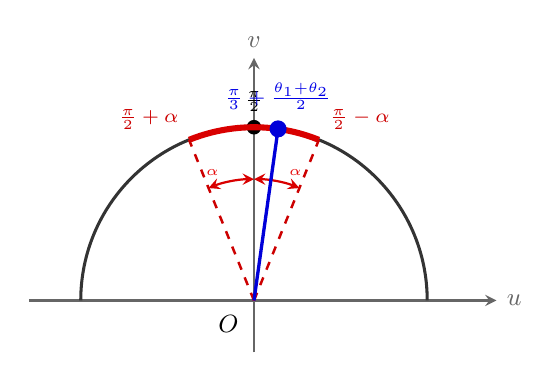
\begin{tikzpicture}[scale=2.2, >=stealth, every node/.style={font=\small}]

    % 座標軸
    \draw[->, thick, gray!80!black] (-1.3, 0) -- (1.4, 0) node[right] {$u$};
    \draw[->, thick, gray!80!black] (0, -0.3) -- (0, 1.4) node[above] {$v$};
    \node[below left=2pt] at (0, 0) {$O$};

    % 単位円上半分
    \draw[line width=1.1pt, gray!40!black] (1, 0) arc (0:180:1);

    % 角 pi/2 (真上: sin = 1)
    \coordinate (Top) at (0, 1);
    \fill[black] (Top) circle (1.2pt);
    \node[above=2pt, font=\scriptsize] at (Top) {$\frac{\pi}{2}$};

    % 許容される偏角の範囲: [pi/2 - alpha, pi/2 + alpha]
    % 視覚化のため alpha を大きめに設定 (例: 22°)
    \def\alPlot{22}
    \coordinate (Pleft)  at ({90 + \alPlot}:1);
    \coordinate (Pright) at ({90 - \alPlot}:1);

    % 範囲の円弧強調 (太い赤線)
    \draw[line width=2.2pt, red!85!black] ({90 - \alPlot}:1) arc ({90 - \alPlot}:{90 + \alPlot}:1);

    % 動径線
    \draw[dashed, red!80!black, line width=0.9pt] (0, 0) -- (Pleft)
    node[above left, font=\scriptsize\bfseries] {$\frac{\pi}{2} + \alpha$};
    \draw[dashed, red!80!black, line width=0.9pt] (0, 0) -- (Pright)
    node[above right, font=\scriptsize\bfseries] {$\frac{\pi}{2} - \alpha$};

    % 角 alpha の補助矢印
    \draw[<->, red!85!black, thick] ({90 - \alPlot}:0.7) arc ({90 - \alPlot}:90:0.7);
    \node[red!90!black, font=\tiny\bfseries, right=1pt] at (80:0.75) {$\alpha$};

    \draw[<->, red!85!black, thick] (90:0.7) arc (90:{90 + \alPlot}:0.7);
    \node[red!90!black, font=\tiny\bfseries, left=1pt] at (100:0.75) {$\alpha$};

    % 角 pi/3 + (theta1+theta2)/2 の代表点
    \coordinate (Pval) at (82:1);
    \fill[blue!85!black] (Pval) circle (1.4pt);
    \draw[line width=1.2pt, blue!85!black] (0, 0) -- (Pval)
    node[above=3pt, font=\scriptsize\bfseries, blue!90!black] {$\frac{\pi}{3} + \frac{\theta_1+\theta_2}{2}$};

  \end{tikzpicture}
  \caption{単位円上における偏角 $\dfrac{\pi}{3} + \dfrac{\theta_1+\theta_2}{2}$ と許容区間の比較}
  \label{fig:angle_comparison_on_unit_circle}
\end{figure}

左辺は\cref{eq:3}より，$\theta$を動かした時に
\begin{align}
  \sin(\dfrac{\pi}{2}\pm \alpha) \le \sin(\dfrac{\pi}{2} - \theta) \le \sin \dfrac{\pi}{2}
\end{align}
の範囲を動く．

右辺については$0 \le \theta_k \le \dfrac{\pi}{3}$ から，
\begin{align}
  \dfrac{1}{6}\pi \le \dfrac{1}{3}\pi + \dfrac{\theta_1 + \theta_2}{2} \le \dfrac{2}{3}\pi
\end{align}
の範囲に納まるから，偏角を比較して$\theta_1+\theta_2$のとりうる範囲は
\begin{align}
  \dfrac{\pi}{2} - \alpha \le \dfrac{1}{3}\pi + \dfrac{\theta_1 + \theta_2}{2} \le \dfrac{\pi}{2} + \alpha \\
  \therefore
  \dfrac{1}{3}\pi - 2\alpha \le \theta_1 + \theta_2 \le \dfrac{1}{3}\pi + 2\alpha \label{eq:6}
\end{align}
である．

\paragraph{(3)}

題意の時，対称性から\cref{eq:6}と同様の式
\begin{align}
  \begin{cases}
    \dfrac{1}{3}\pi - 2\alpha \le \theta_2 + \theta_3 \le \dfrac{1}{3}\pi + 2\alpha \\
    \dfrac{1}{3}\pi - 2\alpha \le \theta_3 + \theta_1 \le \dfrac{1}{3}\pi + 2\alpha
  \end{cases} \label{eq:7}
\end{align}
が成り立つ．\cref{eq:7}の辺々足して
\begin{align}
  \dfrac{2}{3}\pi - 4\alpha \le \theta_1 + \theta_2 + 2\theta_3 \le \dfrac{2}{3}\pi + 4\alpha
\end{align}
で，\cref{eq:6}を引くと
\begin{align}
  \dfrac{1}{6}\pi - 3\alpha \le \theta_3 \le \dfrac{1}{6}\pi + 3\alpha
\end{align}
を得る．対称性から$\theta_1, \theta_2$ についても同様の式が成立し，まとめて
\begin{align}
  \dfrac{1}{6}\pi - 3\alpha \le \theta_k \le \dfrac{1}{6}\pi + 3\alpha \label{eq:8}
\end{align}
である．

$k=1,2,3$に対して
\begin{align}
  \overrightarrow{OP_k(t)} = \overrightarrow{OA_k} + T \vec{e}_k \label{eq:9}
\end{align}
である．
\begin{align}
  |\overrightarrow{OA_k}| = \dfrac{1000}{\sqrt{3}}, |\vec{e}_k|=1
\end{align}
であり，$\beta_k$を$\vec{e}_k$と$\overrightarrow{OA_k}$の成す角とする．
\cref{eq:9}の両辺二乗して，$T=\dfrac{1000}{\sqrt{3}}$に注意すると
\begin{align}
  |\overrightarrow{OP_k(T)}|^2
  &= |\overrightarrow{OA_k}|^2 + T^2 |\overrightarrow{e_k}|^2 + 2T \overrightarrow{e_k} \cdot \overrightarrow{OA_k} \\
  &= \left(\dfrac{1000}{\sqrt{3}}\right)^2 + T^2 + 2T \left(\dfrac{1000}{\sqrt{3}}\right) \cos \beta_k \\
  &= 2T^2(1 + \cos \beta_k) = 4T^2 \cos^2 \dfrac{\beta_k}{2}
\end{align}
より，
\begin{align}
  |\overrightarrow{OP_k(T)}| = 2T \left|\cos \dfrac{\beta_k}{2}\right| \label{eq:10}
\end{align}
が従う．

% TODO: fig, theta_kとbeta_kの関係
% TODO: fig, theta_kとbeta_kの関係 (場合分けを左右に並べた完全版)
\begin{figure}[htb]
  \centering
  % ============================================================
  % 左図: ケース 1° (0 <= theta_2 <= pi/6)
  % ============================================================
  \begin{tikzpicture}[scale=1.1, >=stealth, every node/.style={font=\small}]

    % 正三角形頂点 (A1: 上 90°, A2: 左下 210°, A3: 右下 330°)
    \coordinate (O)  at (0, 0);
    \coordinate (A1) at (90:2.4);
    \coordinate (A2) at (210:2.4);
    \coordinate (A3) at (330:2.4);

    % 正三角形の外枠
    \draw[line width=1.0pt, gray!40] (A1) -- (A2) -- (A3) -- cycle;
    \fill[black] (O) circle (1.2pt) node[above right=1pt, font=\scriptsize] {$O$};

    % 辺 A2A1 (上向き 60°) および 辺 A2A3 (水平 0°)
    \draw[line width=1.1pt, gray!50!black] (A2) -- (A1);
    \draw[line width=1.3pt, gray!20!black, ->] (A2) -- ($ (A2)!0.55!(A3) $)
    node[below=2pt, font=\scriptsize\bfseries] {辺 $A_2A_3$};
    \draw[line width=1.0pt, gray!40] ($ (A2)!0.55!(A3) $) -- (A3);

    % 中心 O への二等分線 (30° = pi/6 の向き)
    \draw[dashed, blue!80!black, line width=0.9pt] (A2) -- (O);
    \draw[->, gray!60!black, line width=0.7pt] ($ (A2) + (0:1.1) $) arc (0:30:1.1);
    \node[gray!70!black, font=\scriptsize\bfseries] at ($ (A2) + (15:1.3) $) {$\frac{1}{6}\pi$};

    % OA2 の向き (左下 -150° = 210°)
    \coordinate (OA2Dir) at ($ (A2) + (-150:0.95) $);
    \draw[line width=1.2pt, teal!85!black, ->] (A2) -- (OA2Dir)
    node[below left=1pt, font=\scriptsize\bfseries] {$\overrightarrow{OA_2}$};
    \node[teal!90!black, font=\tiny\bfseries, above left=1pt] at (OA2Dir) {(\text{8})};

    % 方向ベクトル e2: theta_2 = 16° < 30°
    \def\thTwoA{16}
    \coordinate (e2DirA) at ({\thTwoA}:1);
    \coordinate (B2A)    at ($ (A2) + 1.25*(e2DirA) $);

    \draw[line width=1.5pt, red!85!black, ->] (A2) -- (B2A)
    node[above right=1pt, font=\footnotesize\bfseries] {$\vec{e}_2$};
    \fill[red!85!black] (B2A) circle (1.1pt) node[right=1pt, font=\scriptsize] {$B_2$};

    % 角度円弧
    % (1) theta_2
    \draw[->, thick, red!85!black] ($ (A2) + (0:0.65) $) arc (0:\thTwoA:0.65);
    \node[red!90!black, font=\scriptsize\bfseries] at ($ (A2) + ({\thTwoA/2}:0.85) $) {$\theta_2$};

    % (2) 5pi/6 (OA2 の向きから辺 A2A3 まで)
    \draw[<->, gray!60!black, line width=0.7pt] ($ (A2) + (-150:0.4) $) arc (-150:0:0.4);
    \node[gray!70!black, font=\tiny\bfseries] at ($ (A2) + (-75:0.55) $) {$\frac{5}{6}\pi$};

    % (3) beta_2 = 5pi/6 + theta_2
    \draw[->, line width=1.1pt, teal!90!black]
    ($ (A2) + (-150:0.52) $) arc (-150:{\thTwoA}:0.52);
    \node[teal!95!black, font=\scriptsize\bfseries, fill=white, inner sep=1pt]
    at ($ (A2) + (-65:0.75) $) {$\beta_2 = \frac{5}{6}\pi + \theta_2$};

    % 頂点ラベル
    \fill[black] (A1) circle (1.2pt) node[above=2pt, font=\scriptsize] {$A_1$};
    \fill[black] (A2) circle (1.3pt) node[below=3pt, font=\footnotesize\bfseries] {$A_2$};
    \fill[black] (A3) circle (1.2pt) node[below right=2pt, font=\scriptsize] {$A_3$};

    \node[above, font=\footnotesize\bfseries] at (0, 2.5)
    {$1^\circ\ 0 \le \theta_2 \le \frac{1}{6}\pi$ のとき};

  \end{tikzpicture}
  \quad
  % ============================================================
  % 右図: ケース 2° (pi/6 <= theta_2 <= pi/3)
  % ============================================================
  \begin{tikzpicture}[scale=1.1, >=stealth, every node/.style={font=\small}]

    % 正三角形頂点
    \coordinate (O)  at (0, 0);
    \coordinate (A1) at (90:2.4);
    \coordinate (A2) at (210:2.4);
    \coordinate (A3) at (330:2.4);

    % 正三角形の外枠
    \draw[line width=1.0pt, gray!40] (A1) -- (A2) -- (A3) -- cycle;
    \fill[black] (O) circle (1.2pt) node[above right=1pt, font=\scriptsize] {$O$};

    % 辺 A2A1 (60°) および 辺 A2A3 (0°)
    \draw[line width=1.1pt, gray!50!black] (A2) -- (A1);
    \draw[line width=1.3pt, gray!20!black, ->] (A2) -- ($ (A2)!0.55!(A3) $)
    node[below=2pt, font=\scriptsize\bfseries] {辺 $A_2A_3$};
    \draw[line width=1.0pt, gray!40] ($ (A2)!0.55!(A3) $) -- (A3);

    % 中心 O への二等分線 (30° = pi/6 の向き)
    \draw[dashed, blue!80!black, line width=0.9pt] (A2) -- (O);
    \draw[->, gray!60!black, line width=0.7pt] ($ (A2) + (0:1.1) $) arc (0:30:1.1);
    \node[gray!70!black, font=\scriptsize\bfseries] at ($ (A2) + (15:1.3) $) {$\frac{1}{6}\pi$};

    % OA2 の向き (左下 -150° = 210°)
    \coordinate (OA2Dir) at ($ (A2) + (-150:0.95) $);
    \draw[line width=1.2pt, teal!85!black, ->] (A2) -- (OA2Dir)
    node[below left=1pt, font=\scriptsize\bfseries] {$\overrightarrow{OA_2}$};

    % 方向ベクトル e2: theta_2 = 45° (30° < theta_2 < 60°、二等分線の上側)
    \def\thTwoB{45}
    \coordinate (e2DirB) at ({\thTwoB}:1);
    \coordinate (B2B)    at ($ (A2) + 1.25*(e2DirB) $);

    \draw[line width=1.5pt, red!85!black, ->] (A2) -- (B2B)
    node[above right=1pt, font=\footnotesize\bfseries] {$\vec{e}_2$};
    \fill[red!85!black] (B2B) circle (1.1pt) node[right=1pt, font=\scriptsize] {$B_2$};

    % 角度円弧
    % (1) theta_2 (辺 A2A3 から e2 まで: 45°)
    \draw[->, thick, red!85!black] ($ (A2) + (0:0.65) $) arc (0:\thTwoB:0.65);
    \node[red!90!black, font=\scriptsize\bfseries] at ($ (A2) + (22:0.85) $) {$\theta_2$};

    % (2) 辺 A2A1 (60°) から e2 (45°) までの角: pi/3 - theta_2
    \draw[<->, purple!85!black, thick] ($ (A2) + (60:0.85) $) arc (60:\thTwoB:0.85);
    \node[purple!90!black, font=\tiny\bfseries] at ($ (A2) + (53:1.1) $) {$\frac{\pi}{3} - \theta_2$};

    % (3) beta_2 = 7pi/6 - theta_2 (OA2 と e2 のなす劣角: 時計回りに測る)
    % OA2 (-150°) から時計回り(+) で e2 (45°) までは 360° - (150° + 45°) = 165° = 7pi/6 - theta_2
    \draw[->, line width=1.1pt, teal!90!black]
    ($ (A2) + (-150:0.52) $) arc (-150:{-360 + \thTwoB}:0.52);
    \node[teal!95!black, font=\scriptsize\bfseries, fill=white, inner sep=1pt]
    at ($ (A2) + (135:0.8) $) {$\beta_2 = \frac{7}{6}\pi - \theta_2$};

    % 頂点ラベル
    \fill[black] (A1) circle (1.2pt) node[above=2pt, font=\scriptsize] {$A_1$};
    \fill[black] (A2) circle (1.3pt) node[below=3pt, font=\footnotesize\bfseries] {$A_2$};
    \fill[black] (A3) circle (1.2pt) node[below right=2pt, font=\scriptsize] {$A_3$};

    \node[above, font=\footnotesize\bfseries] at (0, 2.5)
    {$2^\circ\ \frac{1}{6}\pi \le \theta_2 \le \frac{1}{3}\pi$ のとき};

  \end{tikzpicture}
  \caption{頂点 $A_2$ における角 $\theta_2$ と $\beta_2 = \angle(\overrightarrow{OA_2}, \vec{e}_2)$ の場合分け}
  \label{fig:angle_cases_theta2_beta2_side_by_side}
\end{figure}

ここで$\theta_k$と$\beta_k$について上図から
\begin{align}
  \beta_k =
  \begin{cases}
    \dfrac{5}{6}\pi + \theta_k \quad (0 \le \theta_k \le \dfrac{1}{6}\pi) \quad \cdots (8) \\
    \dfrac{7\pi}{6} - \theta_k \quad (\dfrac{1}{6}\pi \le \theta_k \le \dfrac{1}{3}\pi)
  \end{cases} \label{eq:11}
\end{align}
である．

\subparagraph{$1^\circ \ 0 \le \theta_k \le \dfrac{1}{6}\pi$の時}

\cref{eq:8,eq:11}から，$\beta_k$について
\begin{align}
  \dfrac{\pi}{2} - \dfrac{3}{2}\alpha \le \dfrac{\beta_k}{2} \le \dfrac{\pi}{2} + \dfrac{3}{2}\alpha
\end{align}
が成り立つ．両辺$\cos$をとって
\begin{align}
  0 \le \left|\cos \dfrac{\beta_k}{2}\right| \le \left|\cos(\dfrac{\pi}{2} - \dfrac{3}{2}\alpha)\right| = \left|\sin \dfrac{3}{2}\alpha \right| = \sin \dfrac{3}{2}\alpha
\end{align}
である．この右辺について
\begin{align}
  \sin \dfrac{3}{2}\alpha < \sin 2\alpha = 2 \sin \alpha \cos \alpha = \dfrac{2 \sqrt{10^6 - 1}}{10^6} < \dfrac{2}{1000} < \dfrac{3\sqrt{3}}{2000}
\end{align}
だから，\cref{eq:10}より
\begin{align}
  |\overrightarrow{OP_k(T)}| < 2T \dfrac{3\sqrt{3}}{2000} = 3
\end{align}
となり題意は成立する．

\subparagraph{$2^\circ \ \dfrac{1}{6}\pi \le \theta_k \le \dfrac{\pi}{3}$の時}

\cref{eq:8,eq:11}から，$\beta_k$について
\begin{align}
  \dfrac{\pi}{2} - \dfrac{3}{2}\alpha \le \dfrac{\beta_k}{2} \le \dfrac{\pi}{2}
\end{align}
が成り立つ．これは$1^{\circ}$と同様の式だから，この場合も題意は成立する．
\casesend

以上から，たしかに $|\overrightarrow{OP_k(T)}| \le 3$ が $k=1,2,3$ で成立し，題意は示された．
\end{document}
